\documentclass[10pt]{article}
\usepackage{amsmath}
 \usepackage{graphicx}
\usepackage[usenames,dvipsnames]{color}    
\usepackage{listings}
\usepackage[top=1in, bottom=1in, left=1in, right=1in]{geometry}


\lstset{
language=R,                     % the language of the code
  basicstyle=\small\ttfamily, % the size of the fonts that are used for the code
  numbers=none,                   % where to put the line-numbers
  stepnumber=1,                   % the step between two line-numbers. If it's 1, each line
                                  % will be numbered
  numbersep=2pt,                  % how far the line-numbers are from the code
  backgroundcolor=\color{white},  % choose the background color. You must add \usepackage{color}
  showspaces=false,               % show spaces adding particular underscores
  showstringspaces=false,         % underline spaces within strings
  showtabs=false,                 % show tabs within strings adding particular underscores
  frame=none,                   % adds a frame around the code
  tabsize=2,                      % sets default tabsize to 2 spaces
  captionpos=b,                   % sets the caption-position to bottom
  breaklines=true,                % sets automatic line breaking
  breakatwhitespace=false        % sets if automatic breaks should only happen at whitespace
   keywordstyle=\color{RoyalBlue},      % keyword style
    commentstyle=\color{YellowGreen},   % comment style
    stringstyle=\color{ForestGreen},      % string literal style
      numberstyle=\small\color{Blue} % the style that is used for the line-numbers
}
\usepackage{gensymb}
\title{ CS221 Project Progress Report}
\author{How to Succeed with Bitcoin Without Really Trying \\Ellen Sebastian, Abaho Katabarwa, Guoxing Li  }

\begin{document}
\maketitle

 						
 Bitcoin is the world's first decentralized cryptocurrency. Since it was created by Satoshi Nakamoto in 2008, Bitcoin has become a popular international digital payment system because of its ability to bypass national financial regulatory bodies and stay resistant to the fluctuations of traditional currencies. Furthermore, the existence and volatility of bitcoin has created a vibrant and profitable electronic trading market. We would like to take advantage of various concepts in artificial intelligence and the vast amount of transactional data surrounding Bitcoin to create a Bitcoin trading bot whose goal will be to maximize profit by predicting future Bitcoin prices.
 
\section*{Models} 					
 
 
 The problem of maximizing profit can be split into two steps: price change prediction and action selection. Based on the outcome of price change prediction, we can choose an action that maximizes our profit. \\
 Because long-term price prediction is a much harder problem than short-term prediction, we decided to frame the price-prediction step as follows: for any 
 time t, use current and past data to predict $\Delta p$: the price of Bitcoin at $t+dt$. This approach was used with some success\footnote{http://arxiv-web3.library.cornell.edu/pdf/1410.1231v1.pdf}. In this report, we will describe several algorithms for predicting Bitcoin price at $t + dt$.  The success of this model depends on the fact that we can trade very frequently with little overhead cost; in fact, Bitcoin transaction fees are usually no more than 0.5\% of the value traded.\footnote{https://www.bitstamp.net/fee\_schedule/}
 
  \subsubsection*{Price Prediction Method 1: Regression} 					
				
 	\emph{Model}:\\
 	We assume that $\Delta p$ over some dt can be approximated by function of many real-valued features, including previous prices and the log proportion of buy to sell transactions. For example, in the case of linear regression:  y = xB = [price 60 seconds ago, price 120 seconds ago, log buy/sell ratio, transaction frequency…] [B1,B2,B3,B4]. 
 We use a regression algorithm to learn the parameters of such a function and apply the learned function to unseen examples. \\\\
 	\emph{Algorithm}:\\
 For the price prediction stage, consider the date November 11, 2014 and let $dt$ = 60. We choose 1000 random historical time points for which we have feature data. For each time point, we accumulate a vector of features leading up to November 11, 2014, such as the average $\Delta p$ per minute over the last 60 minutes, the same per day over the last 60 days, and log proportion of buy to sell transactions. Using the same input features, we train Linear Regression, Ridge Regression, and Bayesian Ridge Regression on the 1000 time points. We used 10-fold cross-validation to test the algorithm’s performance on unseen data points. We also tried Gaussian Processes Regression.  The use of this specific regression algorithm will be explained in later section.
 
   \subsubsection*{Price Prediction Method 2: Artificial Neural Networks} 					

\emph{Model}:\\
 We modeled the problem as a time series prediction. Given a price data $P = [p = 0, p = 1, ... p = n]$ chronologically arranged from $t = 0$ to $n.$ We can create feature vectors  $a = [pi ... pk]$ where $i >= 0$ and $k < n - 1$ at regular intervals of $P$ and target values $b = pk+1$. \\\\
 	\emph{Algorithm}:\\
 First we initialize our neural network $N$. Given price data  $P = [p = 0, p = 1, ... p = n]$, we determine a window size of $a << |P|$. We then move this window along some interval of $P$ while at each at each iteration using the window to create a feature vector and a target value. Once we have $K$ feature vectors and target values we can train $N$ and predict $pk+1$ given a feature vector $[pk - a ... pk]$.  See appendix item a) for the full code of the algorithm, and appendix item b) for a diagram of the algorithm.\\\\
 	\emph{Example}:\\
 Consider the price data $[.5, .6, .2, .1, 0.01, 0.2]$. We choose a window size of 2 and create the following feature vectors and target pairs $A = [ ([.5, .6], [.6]) ([.6, .2], [.1]) ([.2, .1], [0.01]) ([.1, 0.01], [0.2]) ]$. We can use $A$ to train the neural network $ N$. In order to predict the next data point we input the last feature vector $[0.01, 0.2]$ into $N$.  
  
 
 \subsection*{Action selection}
 
\subsubsection*{Rule-based approach}
 We can use our estimate for the future price of Bitcoin to choose an action that we believe will maximize our profit. These actions are simply, ``do nothing'', ``sell $X$ bitcoins'', or ``buy $X$ bitcoins''. Simple rule-based approaches, such as ``buy when the price will rise more than \$1 in the next hour, sell when the price will drop more than \$1 in the next hour, never sell at a loss'' imitate human decisionmaking and may be successful\footnote{http://arxiv-web3.library.cornell.edu/pdf/1410.1231v1.pdf}.  We will compare the success of a rule-based approach to a policy produced by an MDP.
 	
\subsubsection*{Policy-based approach}										
 In this algorithm, we use Gaussian Processes (GP) and Markov Decision Process (MDP) to model our bitcoin trading problem. The basic idea is to use GP to predict a normal distribution of bitcoin price at the next time step, which can be used to estimate the transition probabilities in our MDP model. We first construct the MDP model based on the following simplified model. Suppose we are given M bitcoins at the beginning, our task is to sell all of them within a fixed time period T, and maximize the revenue we received. Also assume that when we place an order at time T, all of the shares placed will be sold at the average price of that time.
 
\emph{MDP specifications}:
\begin{itemize}
\item States: $(t, b, \Delta p, \sigma)$\\
In the state representation, $t$ means time steps remaining, $b$ means number of bitcoins remaining, $\Delta p$ means the (predicted price - base price) at the next time step, $\sigma$ means the standard deviation of predicted price.
To limit our state space, we discretize each element in our state space. Depending on how large we want our state space to be, we can choose the resolution beforehand. For predicted price, we can define our range by looking at the real price range in the time period that we are interested in. Based on different time step resolution, we adjust the scale of standard deviation accordingly.
\item Actions: \{sell $i$ bitcoins $(0 \leq i < b)$\}\\
The resolution of bitcoin is the same as the one we chose for state space.
��\item $\textrm{Rewards}(s, a, s)$: $-a \times s[\Delta p]$\\
 Rewards are calculated by the amount of bitcoins we chose to sell multiplied by negative predicted price difference (selling bitcoins at the current time step when predicting the price will go up will incur a negative reward).
 \item Transition probabilities: $T(s, a, s'��) \sim N(s[\Delta p], s[\sigma]^2)$\\
 The probability of transition from a state to a new state follows the normal distribution whose mean is $s[\Delta p]$, standard deviation is $s[\sigma]$. Since we are discretizing the states, we take the probability density and normalize it to give us an estimate on the transition probability. It's worth noting that since we don't have information on the transition probability with regard to predicted standard deviation, we assume it stays the same during state transitions.
 \item IsEnd(s): $s[t] = 0$\\
 The simulation ends when time runs out.
 \end{itemize}
 
The framework of this approach is depicted in Figure 1. After constructing the MDP model, we run value iteration on a specific MDP problem by fixing parameters (resolution, price range, etc.), which outputs an optimal policy. When running the simulation, we use GP to generate predictions on the price change as well as its standard deviation at the next time step, which is used to construct a current state and suggests an action based on the optimal policy.
 
\section*{ Results}
 We chose to use different evaluation metrics than we had for the project proposal. In the project proposal, we used the Mean Squared Error on a price prediction; we examined raw price outputs instead of $\Delta p$. Our new results are therefore not comparable with our Oracle and Baseline results.
 	Here, we continue to use Mean Squared error, but instead of examining differences between price predictions, we examine differences between $\Delta p$ predictions. Additionally, we define a crude measure of accuracy in which we consider the algorithm’s classification accuracy between negative and positive changes: 
 	
$ 	 \begin{cases} \text{True positive} &\mbox{if } \Delta p >= 0, \Delta p_{predicted} >= 0 \\ 
\text{False positive} &\mbox{if } \Delta p < 0, \Delta p_{predicted} >= 0 \\ 
\text{True negative} &\mbox{if } \Delta p < 0, \Delta p_{predicted} < 0 \\ 
\text{False negative} &\mbox{if } \Delta p >= 0, \Delta p_{predicted} < 0 \\ 
 	 \end{cases}$ 
 	
 	
 	From the equation above, we can define $accuracy = \frac{TP + TN}{TP + TN + FP + FN}$. This accuracy is our primary evaluation metric. \\
 	
 	All methods of regression performed poorly in predicting $\delta p$.  Accuracy is no better than random in all cases; that is, accuracy $\approx$ 0.5. We hypothesize that this is because Bitcoin prices cannot meaningfully be fit to a function curve; Bitcoin prices in 2014 are not related to those in 2010. Instead, Bitcoin prices depend most heavily on the few days or weeks preding them. \\
 	
 	Gaussian regression shows some promise as a Bitcoin price prediction method. Since GR outputs a mean and standard deviation of our beliefs about the prediction, we decided to evaluate this method by examining whether the true price lay within the 95\% confidence interval of the GR output. 	We found this was the case in 90.2\% of test examples. Notice that the result might not be really indicative on how well the model performs since as we looked through the result, some standard deviation seems too high. However, the confidence interval does seem to cover the actual price most of time which is useful for our MDP problem.\\
 	
 	Neural nets were the most promising approach. In the best case we acheived accuracy=0.67. We also noted that accuracy is highly sensitive to the choice of parameters for the neural net, such as the number of features and window length. We will continue to tweak neural net parameters to acheive maximal accuracy. 
 	\section*{Future Work}
 	
We have eliminated regression as a viable option for price prediction. We will continue to tweak neural net parameters to acheive maximal accuracy. We may also implement a modified version of Bayesian regression for this purpose. \\

In this report, we have not implemented either a rule-based method or MDP for choosing the optimal action given a price prediction. Going forward, we will explore these and other options for choosing the best action, and write a Bitcoin trading bot that tests our findings on the market. \\

 	It is important to note that because we can trade at a high frequency, it is not necessary to have very high prediction accuracy in order to make a profit. Considering the near-intractable nature of Bitcoin price prediction, we are encouraged by the small amount of success we have had thus far.  
 	 
 
 \section*{Appendix}
 \subsection*{a: diagram of neural net}
 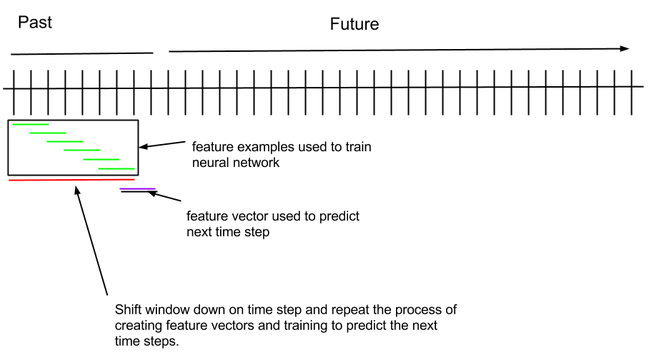
\includegraphics[scale=0.7]{diagram.png}
 \subsection*{b: code for neural net}
 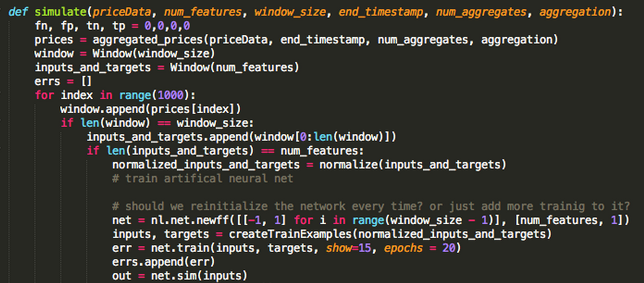
\includegraphics[scale=0.9]{code.png}
 \subsection*{c: performance of 3 regression algorithms in predicting price changes}

 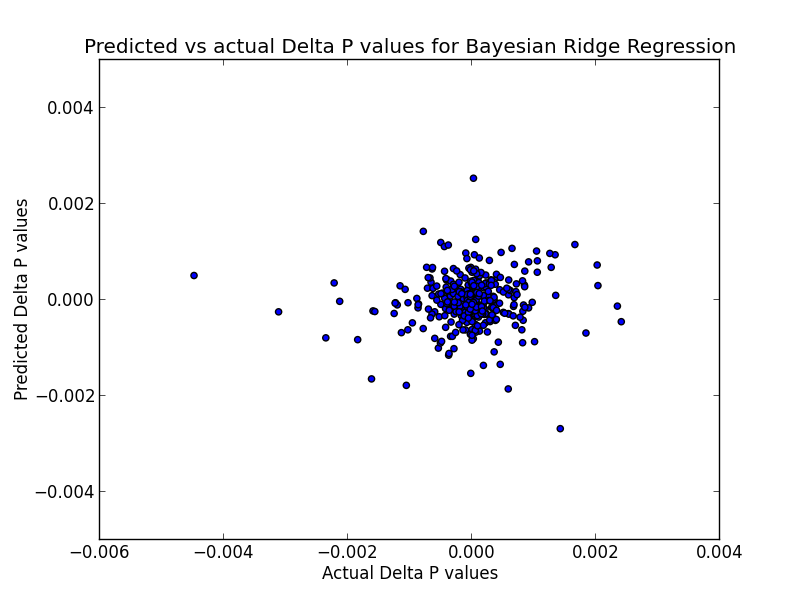
\includegraphics[scale=0.44]{bayesianregression.png}\\

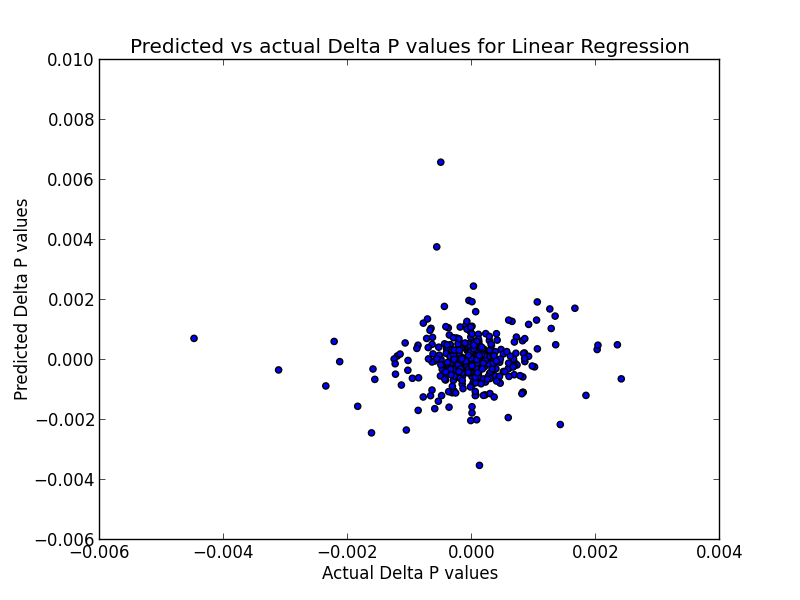
\includegraphics[scale=0.44]{linearregression.png}\\
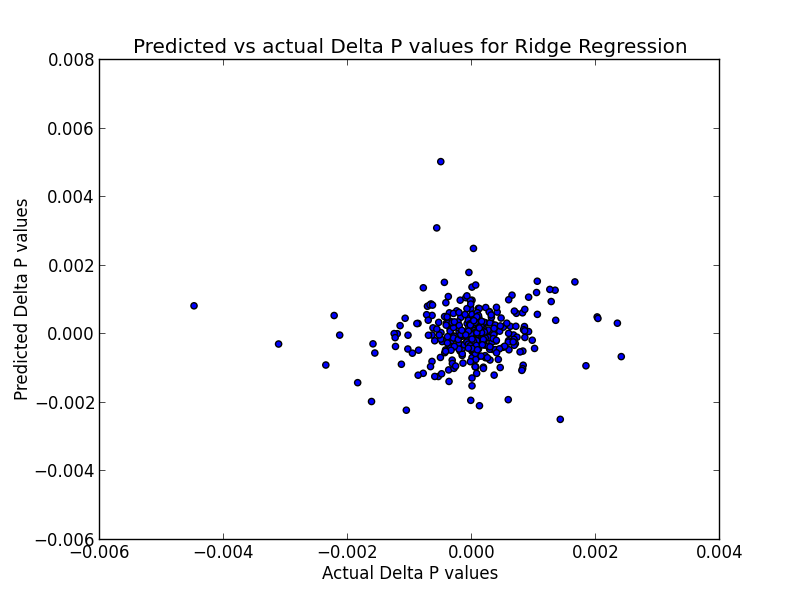
\includegraphics[scale=0.44]{ridgeregression.png}\\
 \end{document}